% !TEX root = template.tex

\begin{table*}[t]
	\begin{center}
		\begin{tabular}{ p{7cm}p{2cm}p{2cm}p{2cm}p{2cm} }
			\hline
			Method & Accuracy & Precision & Recall & F1-Score \\
			\hline
			CNN + No centering & 77.0 & 78.0 & 75.8 & 76.8 \\
			CNN + No centering + Manual F. & 75.6 & 76.8 & 73.9 & 75.3 \\
			CNN + Centering + Manual F. & 86.2 & 86.9 & 70.2 & 77.6 \\
			\textbf{CNN + Centering + Encoder F.} & \textbf{89.2} & \textbf{88.9} &  \textbf{86.1} & \textbf{86.1} \\
			\hline
		\end{tabular}
		\caption{\label{tab:model-performance} UCI classification results with different featueres CNN augumentation and data preprocessing. The test are made with our CNN with OIT, Data centering, 196 (1x16) filters, max-pool (1x4), 64 fully conected, l2-regularization of 5e-5 and Adam learning rate of 2e-5.}
	\end{center}
\end{table*}

\section{Results}
\label{sec:results}

In this section we will present how we selected the appropriate hyper
parameters for the final proposed architecture presented in
Sec. \ref{sec:learning_framework}. Then we will see how some of the
preprocessing blocks and encoder or manual extracted features affect
performance onto the Heterogenity Dataset. We will also shwo results
for the proposed archittecture with OIT applied on Oriented Dataset.

\subsection{Heterogenity Dataset (HD)}

In this section we evaluate performance between previous work and
different model architectures and the influences of some of the
pre-processing techniques applied. Similar to what was done in
\cite{ignatov2018real} we carried out from the HD dataset some
representative users to test the model and then use the remaining ones
to train the model. In this case we selected users \textit{a} and
\textit{b} since we found that they are very representative among all
others. In fact models tend to be less precise with user \textit{a}
and more accurate with user \textit{b}. This mainly depends on the
user's style in walking, doing stairs and so on. In this way we are
able to compare results with other works that usually tend to evaluate
performances on unseen user.

In this training and test set settings, we evaluate the best
hyperparameters for the proposed architecture model excluding OIT
preprocessing block, since this dataset was collected with a fixed
orientation. The rest of pre-processing techinque are enabled, if not
specified.\footnote{FIXME: dovremmo scrivere i risultati per modello piu che per dataset}\\

\textbf{Autoencoder.}  As the Tab.~\ref{tab:ae-loss} confirms, the
Orientation Indipendent Transformation (OIT) is a necessary operation
when dealing with LAR signals. For example, without OIT we can see
that the autoencoder trained and tested on same data goes from
$0.747241$ to $10.421337$ MSE: more than $10$x worse. Furthermore,
data from hand or pocket-up/down do not inflate the loss too
much. This is a good thing because it indicates that autoencoder is
producing robust features.
\begin{table}[H]
  \centering
  \begin{tabular}{lr}
    \hline
    Scenario & Loss (MSE) \\
    \hline
    HD + OIT + OD validation & 0.747241 \\
    HD + OIT + OD validation (allpos) & 0.821241 \\
    HD & 0.871255 \\
    HD + OD validation & 10.421337 \\
    \hline
  \end{tabular}
  \caption{Autoencoder loss on different scenarios}
  \label{tab:ae-loss}
\end{table}

From the grid-search on KNN we suprisingly noticed that performances
do not vary so much on different hyper-parameters: we get from
$76.7$\% to $80.9$\% accuracy. This may be an indication of the
maximum capability of this autoencoder model, so to obtain better
performances we have to add complexity to the model. In particular, we
noticed that KNN usually misclassifies \textit{bike} activity with
\textit{no\textunderscore activity}, in fact \textit{bike} has only
$68$\% precision.

The Tab. \ref{tab:ae-classifiers-accuracy} shows KNN and FFNN accuracy
for the selected autoencoder with $36$ features and the two
classifier described in Sec. \ref{subsec:autoencoder}. Again,
we can see how the OIT is really helpful in our task: without it we
couldn't event reach coin-flip accuracy. Moreover we can say that the
two models are higly correlated in performaces with a difference of
$\approx 10$\% accuracy from KNN to FFNN. The FFNN performs better
than KNN only on \textit{HD} without OIT, but this could be due to
overfitting.

\begin{table}[H]
  \centering
  \begin{tabular}{p{4cm}rr}
    \hline
    Scenario & KNN acc. & FFNN acc. \\
    \hline
    HD + OIT + OD validation & 82.2  & 72.3 \\
    HD + OIT + OD validation (allpos) &  78.9 & 68.0 \\
    HD & 76.2 & 81.8 \\
    HD + OD validation & 27.8 & 10.3 \\
    \hline
  \end{tabular}
  \caption{KNN and FFNN accuracy comparison}
  \label{tab:ae-classifiers-accuracy}
\end{table}

\textbf{CNN Network.} We fist test how number of convolutional filters and number of dense neurons in the FC2 layer will influence classification performances. The results obtained are presented in Tab. \ref{tab:model-selection}. Wee decided to choose 196 convolutional filters and 64 dense neurons thanks to its balance between accuracy and F1-Score performance, obtaining 88.9\% accuracy score and  81.6\%. To compare our result with that obtained in the original work \cite{blunck2013heterogeneity}, we decided to perform their \textit{Leave-one-user-out cross validation} evaluation, consisting of test the model with data from one user, and train with data from all the others in a cross validation fashion and then averaging the metrics obtained. In this evaluation setting we obtained an average F1-score of 85.8\%, beating their best model result of nearly 10\% more of F1-Score metrics. This prove also that using users a and b to do our evaluation is a good compromise of the real \textit{Leave-one-user-out cross validation} evaluation performances, since we obtain nearly the same results (90.2\% instead of 88.9\% in accuracy and 85.8\% instead of 81.6\%). TODO scrivere nelle conslusione che in questo settings abbiamo notato un bel po di varianza tra utenti.

\begin{table}[h]
	\begin{center}
		\begin{tabular}{ p{1.8cm}p{1.7cm}p{1.7cm}p{1.7cm} }
			\hline
			CNN Filters & Dense Neurons & Accuracy & F1-Score \\
			\hline
			196 & 1024 & 84.6 & 75.3 \\
			196 & 512 & 86.1 & 75.7 \\
			\textbf{196} & \textbf{64} & \textbf{88.9} & \textbf{81.6} \\
			96 & 1024 & 82.8 & 69.9 \\
			96 & 512 & 84.4 & 73.7 \\
			96 & 64 & 89.0 & 73.0 \\
			48 & 1024 & 80.0 & 79.4 \\
			48 & 512 & 83.7 & 74.9 \\
			48 & 64 & 84.0 & 72.3 \\
			\hline
		\end{tabular}
		\caption{\label{tab:model-selection} UCI classification results with data centering and manual features augmented CNN}
	\end{center}
\end{table}


To better appreciate how our pre-processing block affects model overall performance, we also try to disable or enable some of these blocks. In Tab. \ref{tab:model-performance} we report our obtained results experiments. We see that augmenting the CNN with manual extracted feature when data are not centered, lead to no significant change in performances, instead when also enable data centering pre-processing with manual features augmented CNN the model obtain nearly 10\% more in accuracy and precision metrics. This prove the benefits of data centering stated previously. However we were not able to get the same performances obtained in \cite{ignatov2018real}, where the authors obtained in the same exact setting an accuracy of 97.6\%. These empirically confirm that performances of state-of-the-art models trained with one type of sensors are worse when dealing with smartphone sensor heterogeneity. Moving on, augmenting the CNN with encoder feature lead the model to better performances, meaning that encoder feature are more robust that manual feature, as explained previously. A confusion matrix in this latter setting is reported in Fig. \ref{fig:cnn-confusion-matrix} where we could see that the model perform nicely overall in all the considered activities, with some difficulties in distinguishing between stationary activities, stand and sit, and walk activity with stairs since that activities are very similar in sensor signals foot-prints.

\begin{figure}[h]
	\centering
	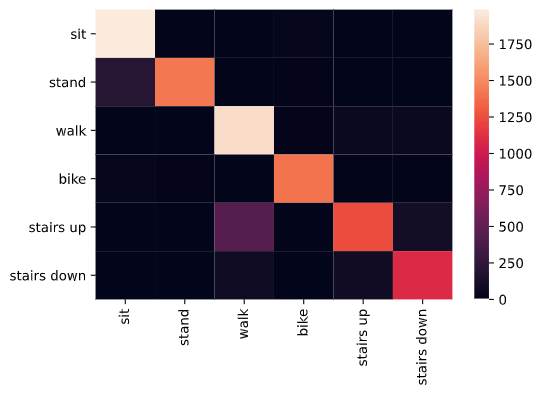
\includegraphics[width=0.5\textwidth]{images/confusion_matrix.png}
	\caption{CNN confusion matrix}
	\label{fig:cnn-confusion-matrix}
\end{figure}


\subsection{Oriented Dataset (OD)}

The Tab. \ref{tab:model-performance} shows how the model behaves on
the new unseen data from \textit{OD} where LAR signals are collected
in different orientations. The first thing to nitice is that results
really benefit from OIT: with phone in pouch we were able to obtain
$85.3$\% accuracy. The model performs decently even on data from hand
and pocket where signals have lot of noise, though we have a slight
worsening. Furthermore, we got $78.0$\% accuracy on full \textit{OD},
i.e., more or less the mean between pouch and hand/pocket results.

\begin{table}[ht]
  \begin{center}
    \begin{tabular}{p{1.8cm}rrrr}
      \hline
      Positions & Accuracy & Precision & Recall & F1-score \\
      \hline
      Pouch & 85.3 & 92.0 & 73.8 & 81.9 \\
      Hand+Pocket & 70.5 & 79.5 & 63.0 & 70.2 \\
      All & 78.0 & 84.0 & 69.0 & 75.7 \\
      \hline
    \end{tabular}
    \caption{Classification comparisons onto \textit{OD} between
      smartphone positions (pouch left/right/top/back, hand and
      pocket-up/down and all positions).}
    \label{tab:model-performance}
  \end{center}
\end{table}


